% !TEX program = lualatex
% Compile from 2026/week9; figures are reproduced by make_figures.py.
\documentclass[12pt,aspectratio=43]{beamer}
% Shared Beamer design. Load after \documentclass using \input.
% Engine: LuaLaTeX. Fonts: UD Digi Kyokasho N (regular/bold), Arial.
\usepackage{luatexja-fontspec}
\setmainjfont[BoldFont={UD Digi Kyokasho N Bold}]{UD Digi Kyokasho N}
\setsansjfont[BoldFont={UD Digi Kyokasho N Bold}]{UD Digi Kyokasho N}
\setmonojfont[BoldFont={UD Digi Kyokasho N Bold}]{UD Digi Kyokasho N}
% Liberation Sans keeps the layout usable on systems without Arial.
\IfFontExistsTF{Arial}{
  \setmainfont{Arial}
  \setsansfont{Arial}
  \setmonofont{Arial}
}{
  \setmainfont{Liberation Sans}
  \setsansfont{Liberation Sans}
  \setmonofont{Liberation Sans}
}
\renewcommand{\kanjifamilydefault}{\gtdefault}

% Typeset mathematics with a dedicated TeX math font, independent of Arial.
\usefonttheme{professionalfonts}
\usepackage[mathrm=sym]{unicode-math}
\setmathfont{Latin Modern Math}
\setoperatorfont{\symup}

\definecolor{courseblue}{HTML}{4472C4}
\definecolor{ruleblue}{HTML}{8FAADC}
\setbeamercolor{normal text}{fg=black,bg=white}
\setbeamercolor{structure}{fg=courseblue}
\setbeamercolor{frametitle}{fg=black,bg=white}
\setbeamercolor{title banner}{fg=white,bg=courseblue}
\setbeamerfont{frametitle}{size=\fontsize{18}{22}\selectfont,series=\mdseries}
\setbeamerfont{quote}{shape=\upshape}
\setbeamersize{text margin left=9mm,text margin right=9mm}
\setbeamertemplate{navigation symbols}{}
\setbeamercolor{page number}{fg=gray,bg=white}
\setbeamertemplate{footline}{%
  \begin{beamercolorbox}[wd=\paperwidth,ht=2.5mm,dp=1.5mm]{page number}
    \hfill{\fontsize{8}{9}\selectfont
      \ifnum\value{framenumber}>0
        \insertframenumber\,/\,\inserttotalframenumber
      \fi}\hspace*{3mm}
  \end{beamercolorbox}}
\setbeamertemplate{headline}{%
  \hfill\textcolor{gray}{\fontsize{6}{7}\selectfont
    \hypersetup{linkcolor=gray}% Keep Beamer's title links in the header color.
    \ifnum\value{framenumber}=0 \insertshortdate\enspace\fi
    \insertshorttitle\space\insertshortsubtitle}\hspace{2mm}\vspace{1.5mm}}
\setbeamertemplate{frametitle}{%
  \vspace{2mm}\centering\insertframetitle\par
  \vspace{-1mm}{\color{ruleblue}\rule{.44\paperwidth}{.5pt}}\par
  \vspace{2mm}}
\setbeamercolor{itemize item}{fg=courseblue}
\setbeamercolor{itemize subitem}{fg=black}
\setbeamercolor{itemize subsubitem}{fg=black}
\setbeamertemplate{itemize item}{\textbullet}
\setbeamertemplate{itemize subitem}{\textnormal{-}}
\setbeamertemplate{itemize subsubitem}{\textnormal{-}}
\setlength{\parskip}{.45em}
\hypersetup{colorlinks=true,urlcolor=courseblue}

% Use \titlepage inside a [t,noframenumbering] frame. The background extends
% 1 mm past both page edges to avoid hairline gaps in PDF viewers.
\setbeamertemplate{title page}{%
  \vspace{2mm}
  \begin{beamercolorbox}[wd=\paperwidth,ht=43mm,dp=13mm,colsep*=1mm,center]{title banner}
    {\fontsize{32}{40}\selectfont\inserttitle\par}
    \vspace{2mm}
    {\fontsize{20}{24}\selectfont\insertsubtitle\par}
  \end{beamercolorbox}
  \vspace{10mm}
  \hfill\insertauthor
}

\graphicspath{{figures/}}
\usepackage{listings}
\usepackage{upquote}
\IfFontExistsTF{Consolas}{\newfontfamily\codefont{Consolas}}{\newfontfamily\codefont{Liberation Mono}}
\definecolor{codevalue}{HTML}{7A3E9D}
\definecolor{codebuiltin}{HTML}{006DB0}
\definecolor{codestring}{HTML}{267348}
\newcommand{\code}[1]{{\codefont #1}}
\lstdefinestyle{python}{
  language=Python,
  basicstyle=\codefont\fontsize{12}{14}\selectfont,
  keywordstyle=\color{codebuiltin},
  keywordstyle=[2]\color{codebuiltin},
  morekeywords=[2]{print,range},
  stringstyle=\color{codestring},
  showstringspaces=false,
  columns=fullflexible,
  keepspaces=true,
  upquote=true,
  tabsize=4,
  breaklines=false,
  backgroundcolor=\color{black!4},
  frame=single,framerule=0pt,framesep=1.7mm,
  xleftmargin=1.7mm,xrightmargin=1.7mm,
  aboveskip=1mm,belowskip=0.5mm,
  literate=*{0}{{{\color{codevalue}0}}}1
    {1}{{{\color{codevalue}1}}}1 {2}{{{\color{codevalue}2}}}1
    {3}{{{\color{codevalue}3}}}1 {4}{{{\color{codevalue}4}}}1
    {5}{{{\color{codevalue}5}}}1 {6}{{{\color{codevalue}6}}}1
    {7}{{{\color{codevalue}7}}}1 {8}{{{\color{codevalue}8}}}1
    {9}{{{\color{codevalue}9}}}1
}
\lstset{style=python}
\setbeamercolor{lesson note}{fg=black,bg=courseblue!9}
\newenvironment{lessonbox}
  {\begin{beamercolorbox}[wd=\linewidth,sep=1.5mm]{lesson note}}
  {\end{beamercolorbox}\par}

\title{計算物理学B}
\subtitle{第九回：モンテカルロ法2}
\author{野垣 康介、藤本 悠輝}
\date{2026/12/15}
\hypersetup{pdftitle={計算物理学B 第九回：モンテカルロ法2},pdfauthor={野垣 康介、藤本 悠輝}}

\begin{document}

\begin{frame}[t,noframenumbering]
  \titlepage
\end{frame}

\begin{frame}[t]{講義予定}
  \begingroup
  \setlength{\tabcolsep}{1.6mm}
  \renewcommand{\arraystretch}{1.25}
  \begin{tabular}{@{}l@{\hspace{2mm}}l@{\hspace{4mm}}l@{\hspace{2mm}}l@{}}
    10/6 & 四則演算 & 12/8 & モンテカルロ1 \\
    10/27 & 制御文（for, if） & \textcolor{courseblue}{\textbf{12/15}} &
      \textcolor{courseblue}{\textbf{モンテカルロ2}} \\
    11/6（金） & 関数 & 12/22 & 微分方程式1 \\
    11/10 & 配列（NumPy） & 1/12 & 微分方程式2 \\
    11/17 & 可視化（matplotlib） & 1/19 & 偏微分方程式1 \\
    11/24 & 数値微分 & 1/26 & 偏微分方程式2 \\
    12/1 & 数値積分 & 2/2 & 根の探索 \\
    \multicolumn{2}{c}{\small 〜中間レポート〜} &
    \multicolumn{2}{c}{\small 〜期末レポート〜}
  \end{tabular}\par
  \endgroup
  \vspace{2mm}
  {\small 10/20は出張で休講。11/6（金）は火曜授業の振替。\par}
\end{frame}

\begin{frame}[t]{今日の内容}
  \begin{itemize}
    \setlength{\itemsep}{3mm}
    \item Metropolis法をIsing模型に適用する
    \item スピン反転のエネルギー差と受理確率を計算する
    \item 自己相関、熱平衡化、測定間隔を区別する
    \item 磁化の温度依存性をシミュレーションする
  \end{itemize}
\end{frame}

\begin{frame}[t]{Notebookを開く}
  \begin{itemize}
    \setlength{\itemsep}{2.5mm}
    \item Google Colab：\small\url{https://colab.research.google.com/?hl=ja}
    \item GitHub：\small\href{https://github.com/nogaki/Computational_Physics_B/tree/main/2026/week9/week9.ipynb}{2026/week9/week9.ipynb}
    \item Colabの「ファイル」\(\to\)「ノートブックを開く」\(\to\)「GitHub」から開く
  \end{itemize}
  \vspace{2mm}
  \begin{lessonbox}
    \textbf{開いたら「ドライブにコピーを保存」}\par
    \small GitHub上のNotebookを開いただけでは、自分のDriveには保存されません。
  \end{lessonbox}
  \vspace{2mm}
  \small 実行前に上から順にセルを動かし、乱数seedと計算回数を確認します。
\end{frame}

\begin{frame}[t]{Metropolis法：目標分布から標本を作る}
  \begin{itemize}
    \setlength{\itemsep}{2mm}
    \item 目標分布 $P(x)$ の形は分かるが、そこから直接乱数を作れない場合を考える
    \item 提案 $x'\sim q(x'|x)$ を作り、受理確率で次の状態を決める
  \end{itemize}
  \[
    a(x\to x')=\min\!\left(1,
      \frac{P(x')q(x|x')}{P(x)q(x'|x)}\right)
  \]
  \begin{lessonbox}
    対称な提案 $q(x'|x)=q(x|x')$ なら
    $a=\min(1,P(x')/P(x))$。
    熱平衡分布 $P\propto e^{-\beta H}$ では
    $a=\min(1,e^{-\beta\Delta E})$。
  \end{lessonbox}
\end{frame}

\begin{frame}[t]{Ising模型}
  \begin{columns}[T,onlytextwidth]
    \column{0.61\textwidth}
    \begin{itemize}
      \setlength{\itemsep}{2mm}
      \item 格子点ごとにスピン $s_i=\pm1$
      \item 最近接相互作用 $J>0$ は平行スピンを好む
      \item 外場 $h=0$、正方格子、周期境界を考える
    \end{itemize}
    \[
      H=-J\sum_{\langle ij\rangle}s_i s_j
        -h\sum_i s_i,
      \qquad h=0
    \]
    \column{0.35\textwidth}
    \centering
    \renewcommand{\arraystretch}{1.6}
    \begin{tabular}{c|c|c}
      $+1$ & $+1$ & $-1$ \\
      \hline
      $+1$ & $-1$ & $-1$ \\
      \hline
      $-1$ & $+1$ & $+1$
    \end{tabular}
    \par\small スピン配位の一例
  \end{columns}
  \vspace{1mm}
  \small $k_{\rm B}$ はBoltzmann定数。計算では $J=k_{\rm B}=1$ とし、温度は $k_{\rm B}T/J$ で表す。
\end{frame}

\begin{frame}[t]{次元と相転移}
  \begin{itemize}
    \setlength{\itemsep}{3mm}
    \item 1次元Ising模型：有限温度では長距離秩序を持たない
    \item 2次元正方格子・$h=0$：厳密解があり、有限温度で相転移
    \item 3次元以上：一般に厳密解は得られず、数値計算が重要
  \end{itemize}
  \begin{lessonbox}
    2次元正方格子では
    $\displaystyle \frac{k_{\rm B}T_c}{J}
      =\frac{2}{\ln(1+\sqrt2)}\simeq2.269$。
    $T<T_c$ で強磁性、$T>T_c$ で常磁性。
  \end{lessonbox}
\end{frame}

\begin{frame}[t]{配位の数と磁化}
  \begin{itemize}
    \setlength{\itemsep}{2mm}
    \item $N$ 個のスピンの配位数は $2^N$。全配位の列挙は大規模系で困難
    \item Monte Carlo法は熱平衡分布に従う配位を標本化する
  \end{itemize}
  \[
    m=\frac{1}{N}\sum_{i=1}^{N}s_i,
    \qquad
    \langle A\rangle=\sum_{\{s_i\}} P(\{s_i\})A(\{s_i\})
  \]
  \begin{lessonbox}
    有限系・$h=0$ では対称性により $\langle m\rangle=0$ になり得る。
    秩序の大きさには $\langle|m|\rangle$ を使う。
    $|\langle m\rangle|$ とは別の量。
  \end{lessonbox}
\end{frame}

\begin{frame}[t]{1回のスピン反転}
  格子点 $i$ のスピン $s_i$ を反転すると、4近傍との結合だけが変わる。
  \[
    \Delta E=E_{\rm after}-E_{\rm before}
      =2J s_i\sum_{j\in\mathrm{nn}(i)}s_j
  \]
  \vspace{-1mm}
  \begin{itemize}
    \setlength{\itemsep}{1.5mm}
    \item $\Delta E<0$：確率1で受理
    \item $\Delta E>0$：確率 $e^{-\beta\Delta E}$ で受理
    \item $\beta=1/(k_{\rm B}T)$。周期境界では端から反対側へつなぐ
  \end{itemize}
  \[
    P_{\rm acc}=\min(1,e^{-\beta\Delta E})
  \]
\end{frame}

\begin{frame}[t,fragile]{Metropolis更新}
  \small 一様にサイトを選び、$\Delta E$ と $P_{\rm acc}$ で反転を決める。
  \vspace{1mm}
  \begin{lstlisting}
i, j = rng.integers(L, size=2)
dE = flip_energy_change(S, i, j)
accept = dE <= 0
if not accept:
    p = np.exp(-beta * dE)
    accept = rng.random() < p
if accept:
    S[i, j] *= -1
  \end{lstlisting}
  \small 1回は1試行。慣例的に $L^2$ 試行を1 Monte Carlo sweepと呼ぶ。
\end{frame}

\begin{frame}[t]{自己相関}
  Markov連鎖が作る配位は、隣接する時刻で似ていることがある。
  \[
    C_A(\ell)=\frac{\langle(A_t-\langle A\rangle)
      (A_{t+\ell}-\langle A\rangle)\rangle}
      {\langle(A_t-\langle A\rangle)^2\rangle}
  \]
  \begin{itemize}
    \setlength{\itemsep}{2mm}
    \item 相関の強い測定値を、独立標本として誤差評価してはいけない
    \item 転移点近くでは相関時間が長くなりやすい
    \item 受理率は自己相関時間そのものではない
  \end{itemize}
\end{frame}

\begin{frame}[t]{熱平衡化と測定間隔は別}
  \begin{columns}[T,onlytextwidth]
    \column{0.48\textwidth}
    \textbf{バーンイン}
    \begin{itemize}
      \item 初期配位の影響を減らす
      \item 先頭の区間を測定から除く
      \item 収束の確認は別途必要
    \end{itemize}
    \column{0.48\textwidth}
    \textbf{自己相関への対処}
    \begin{itemize}
      \item 平衡後の系列から $C_A(\ell)$ を調べる
      \item 測定を間引いても独立とは限らない
      \item 推定した相関時間と有効標本数を使う
    \end{itemize}
  \end{columns}
  \vspace{2mm}
  \begin{lessonbox}
    $L^2/\langle\mathrm{accept}\rangle$ は「全サイトが一度ほど受理される」粗い目安。
    独立配位の間隔を与える式ではない。
  \end{lessonbox}
\end{frame}

\begin{frame}[t]{低温でのスピン配位}
  \centering
  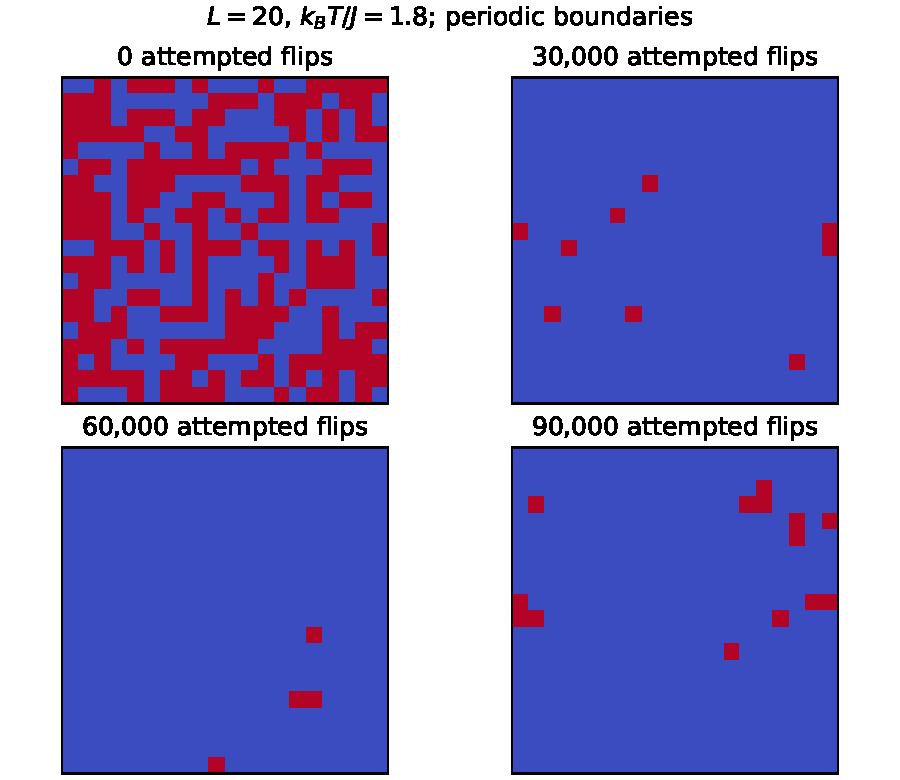
\includegraphics[width=0.54\linewidth]{ising_snapshots.pdf}

  \small $L=20$、$k_{\rm B}T/J=1.8$、ランダムな初期配位。
  \quad 1試行ごとに1サイトを選ぶ。
\end{frame}

\begin{frame}[t]{臨界温度付近の磁化系列}
  \centering
  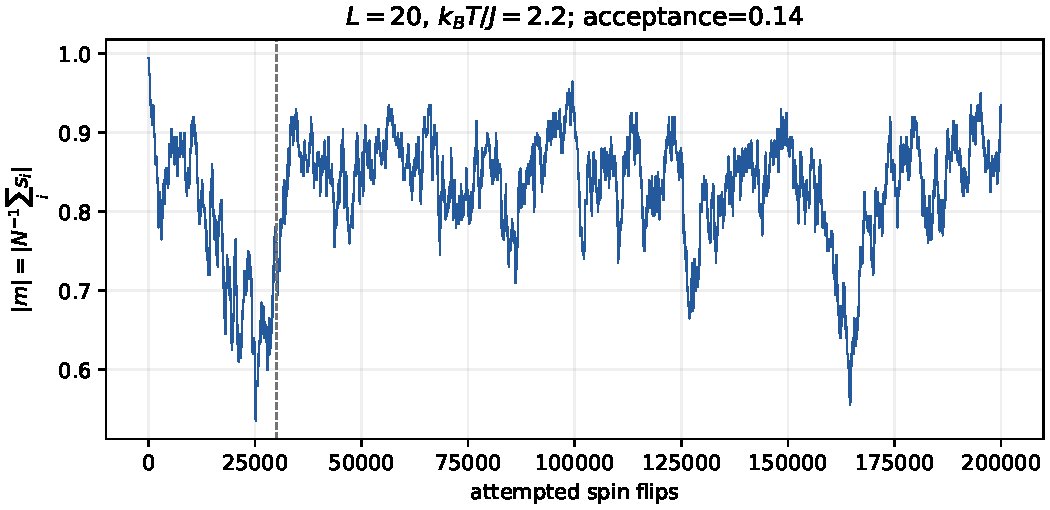
\includegraphics[width=0.88\linewidth]{magnetization_trace.pdf}

  \small $L=20$、$k_{\rm B}T/J=2.2$。破線は例示的なバーンイン境界であり、
  平衡到達を証明する印ではない。
\end{frame}

\begin{frame}[t]{2次元Ising模型の自発磁化}
  \begin{itemize}
    \item 無限正方格子、外場ゼロでの自発磁化
  \end{itemize}
  \[
    m(T)=\left[1-\sinh^{-4}\!\left(\frac{2J}{k_{\rm B}T}\right)\right]^{1/8},
    \qquad m(T\ge T_c)=0
  \]
  \begin{lessonbox}
    $T_c$ は $k_{\rm B}T_c/J=2/\ln(1+\sqrt2)$。
    有限サイズでは磁化の変化が丸まり、臨界点の非解析性は現れない。
  \end{lessonbox}
\end{frame}

\begin{frame}[t]{有限格子の磁化を測る}
  \centering
  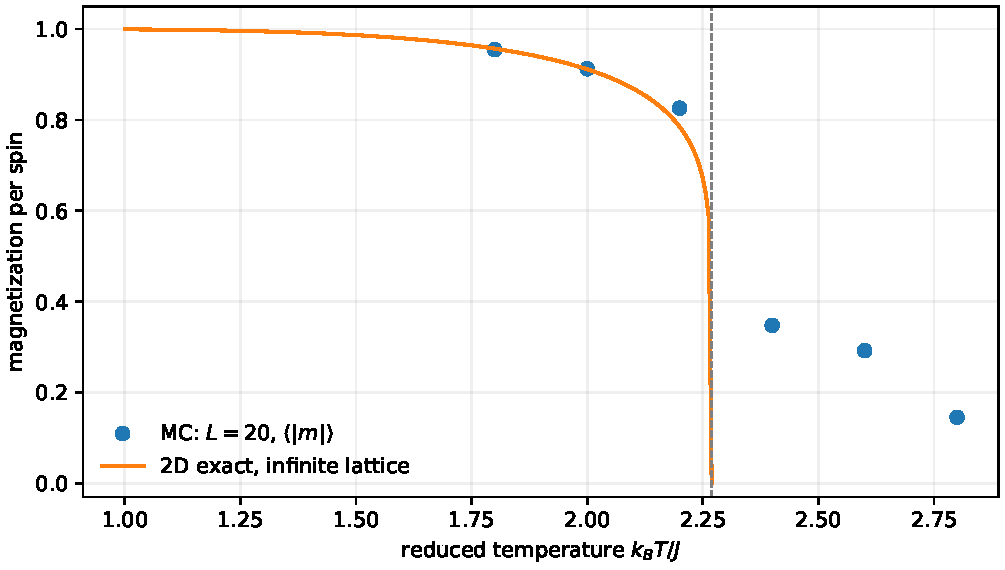
\includegraphics[width=0.78\linewidth]{ising_magnetization.pdf}

  \small $L=20$ の有限時間推定値は、統計揺らぎと有限サイズ効果を含む。
  \quad 臨界点の精密推定には使わない。
\end{frame}

\begin{frame}[t]{演習：磁化の揺らぎと比熱}
  温度ごとに平衡後の標本を集め、次を求める。
  \begin{itemize}
    \setlength{\itemsep}{2mm}
    \item 磁化の二乗平均 $\langle m^2\rangle$
    \item 1スピンあたりの比熱
  \end{itemize}
  \[
    \frac{C_V}{N}=\frac{\beta^2}{N}
       \left(\langle H^2\rangle-\langle H\rangle^2\right)
  \]
  \begin{lessonbox}
    $m$ の平均、$|m|$ の平均、$m^2$ の平均は異なる。
    エネルギー $H$ は全系の値として分散を計算し、最後に $N$ で割る。
  \end{lessonbox}
\end{frame}

\begin{frame}[t]{実習の進め方}
  \begin{enumerate}
    \setlength{\itemsep}{2.5mm}
    \item seedを固定して $L=20$ の更新系列を実行する
    \item $m$ と $|m|$ を並べ、初期区間の影響を見る
    \item 複数温度で $\langle|m|\rangle$ を推定する
    \item $\langle m^2\rangle$ と比熱のセルを埋める
  \end{enumerate}
  \vspace{2mm}
  \small コードの試行回数を短くすると、実行は速くなるが統計誤差は大きくなる。
\end{frame}

\end{document}
